\documentclass{exam}
\usepackage[brazil]{babel}
\usepackage[utf8]{inputenc}
\usepackage{fancyvrb}
\usepackage[pdftex]{geometry}
\geometry{a4paper,left=2cm,right=2.5cm,top=2cm,bottom=2cm}
\usepackage{color}
\usepackage{graphicx}
\usepackage{wrapfig}
\usepackage{comment}
\usepackage{longtable}
\usepackage{multicol}
\usepackage{enumitem}
\usepackage{float}

\pagestyle{empty} % use if page numbers not wanted

\begin{document}
\begin{center}
\vspace*{1cm}
\LARGE \textbf{Prova Enade 2005\\CC \\}\vspace*{0.5cm}
\Large Leia com atenção as instruções a seguir
\vspace*{0.5cm}
\end{center}

\begin{enumerate}
    \item Verifique se, além deste Caderno, você recebeu o Cartão Resposta, destinado à transcrição das respostas das questões de múltipla escolha, das questões discursivas (D) e das questões de percepção da prova.
    \item Confira se este Caderno contém as questões discursivas e as objetivas de múltipla escolha, de formação geral e de componente específico da área, e as relativas à sua percepção da prova. As questões estão assim distribuídas:
REPRODUZIR A TABELA
    \begin{itemize}

        \item Formação Geral: Discursivas (2 questões)\\
        \item Formação Geral: Objetivas  (8 questões)\\
        \item Componente Específico: Discursivas (3 questões)\\
        \item Componente Específico: Objetivas (27 questões)\\
    \end{itemize}

    \item  Verifique se a prova está completa e se o seu nome está correto no Cartão Resposta. Caso contrário, avise imediatamente ao Chefe de Sala.
    \item Assine o Cartão Resposta no local apropriado, com caneta esferográfica de tinta preta, fabricada em material transparente.
    \item As respostas da prova objetiva, da prova discursiva e do questionário de percepção da prova deverão ser transcritas, com caneta esferográfica de tinta preta, fabricada em material transparente, no Cartão Resposta que deverá ser entregue ao Chefe de Sala ao término da prova.
    \item Responda cada questão discursiva em, no máximo, 15 linhas. Qualquer texto que ultrapasse o espaço destinado à resposta será desconsiderado.
    \item Você terá quatro horas para responder às questões de múltipla escolha, às questões discursivas e ao    questionário de percepção da prova.
    \item  Ao terminar a prova, acene para o Chefe de Sala e aguarde-o em sua carteira. Ele então irá proceder à sua identificação, recolher o seu material de prova e coletar a sua assinatura na Lista de Presença.
    \item Atenção! Você deverá permanecer na sala de aplicação por, no mínimo, uma hora a partir do início da prova e só poderá levar este Caderno de Prova quando faltarem 30 minutos para o término do Exame.

\end{enumerate}

\begin{questions}

\question (\textbf{Enade}$|$\textbf{CC}-\textbf{2005}) Está em discussão, na sociedade brasileira, a possibilidade de uma
reforma política e eleitoral. Fala-se, entre outras propostas, em
financiamento público de campanhas, fidelidade partidária, lista
eleitoral fechada e voto distrital. Os dispositivos ligados à
obrigatoriedade de os candidatos fazerem declaração pública de
bens e prestarem contas dos gastos devem ser aperfeiçoados, os
órgãos públicos de fiscalização e controle podem ser equipados
e reforçados.
Com base no exposto, mudanças na legislação eleitoral poderão
representar, como principal aspecto, um reforço da
	\begin{enumerate}[label=\alph*)]
		\item  política, porque garantirão a seleção de políticos experientes e idôneos. 
		\item  economia, porque incentivarão gastos das empresas públicas e privadas. 
		\item  moralidade, porque inviabilizarão candidaturas despreparadas intelectualmente. 
		\item  ética, porque facilitarão o combate à corrupção e o estímulo à transparência. 
		\item  cidadania, porque permitirão a ampliação do número de cidadãos com direito ao voto.  
	\end{enumerate}

\question (\textbf{Enade}$|$\textbf{CC}-\textbf{2005}) Leia e relacione os textos a seguir.
O Governo Federal deve
promover a inclusão digital, pois
a falta de acesso às tecnologias
digitais acaba por excluir
socialmente o cidadão, em
especial a juventude.
\begin{figure}[Hhtb]
	\begin{center}
		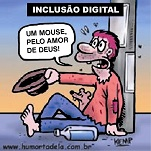
\includegraphics[width=0.5\textwidth]{CIENCIA_DA_COMPUTACAO_Prova2005-utf8_figuras/fig-0001.jpg}
		\caption{Projeto Casa Brasil de inclusão digital começa em 2004. In: Mariana Mazza. JB online.}
	\end{center}
\end{figure}

Comparando a proposta acima com a charge, pode-se concluir que
	\begin{enumerate}[label=\alph*)]
		\item  o conhecimento da tecnologia digital está democratizado no Brasil. 
		\item  a preocupação social é preparar quadros para o domínio da informática. 
		\item  o apelo à inclusão digital atrai os jovens para o universo da computação. 
		\item  o acesso à tecnologia digital está perdido para as comunidades carentes. 
		\item  a dificuldade de acesso ao mundo digital torna o cidadão um excluído social.
	\end{enumerate}

\end{questions}
\end{document}
